\section{Filtrage et compléments sous OpenCV}

\subsection{Etude de quelques filtres usuels}

\subsubsection{Filtre moyenneur}

Un filtre effectue une opération mathématique, appelé convolution, sur un ensemble de données en entrée afin de former
une image de sortie différente. Nous avons appliqué un premier filtre linéaire sur l'image phare.png dont le masque est 
$\begin{pmatrix}
   1 & 1 & 1\\
   1 & 1 & 1\\
   1 & 1 & 1
\end{pmatrix}$.

\begin{figure}[H]
      \center
      \fbox{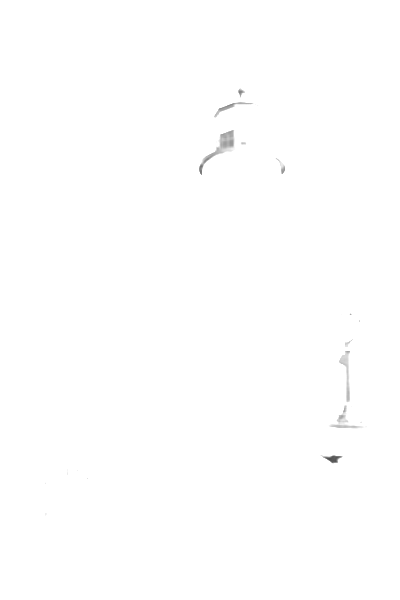
\includegraphics[width=5cm]{ressources/tp4/phare_dest1.png}}
      \caption{Résultat du premier filtre appliqué sur l'image phare.png}
\end{figure}

On peut voir que le résutlat est une image presque totalement blanche. En effet, chaque pixel aura comme valeur la somme
des huit pixels autour de lui. Presque tous les pixels ont alors une valeur supérieure à 255.\\

La normalisation fait en sorte que la somme des valeurs de la matrice fournie soit égale à 1. Nous avons appliqué une normalisation sur 
la matrice précédente, ce qui nous donne une image floutée par rapport au phare.png. Ce flou est encore plus important lorsque
la normalisation se fait sur une matrice de plus grande taille.\\

\begin{figure}[H]
      \center
      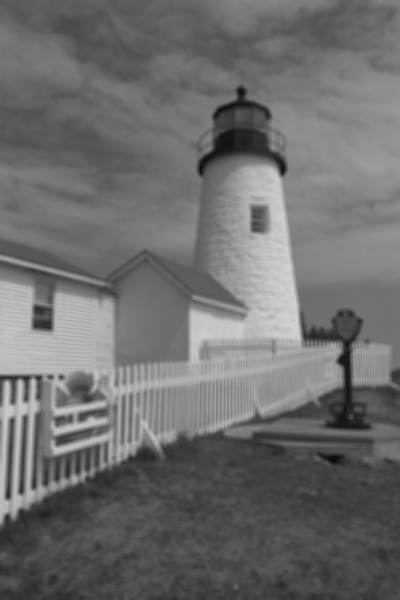
\includegraphics[width=5cm]{ressources/tp4/phare_dest_5x5.png}
      \caption{Résultat de la normalisation avec une matrice 5x5 sur l'image phare.png}
\end{figure}

\subsubsection{Filtre médian}

Le filtre médian consiste à prendre la valeur médiane parmi l'ensemble des huit valeurs autour du pixel traité.
Cela permet, entre autres, d'améliorer la qualité d'une image comportant un bruit assez important. Nous avons testé
ce filtre sur une image avec un bruit de type ``poivre et sel''.

\begin{figure}[H]
      \center
      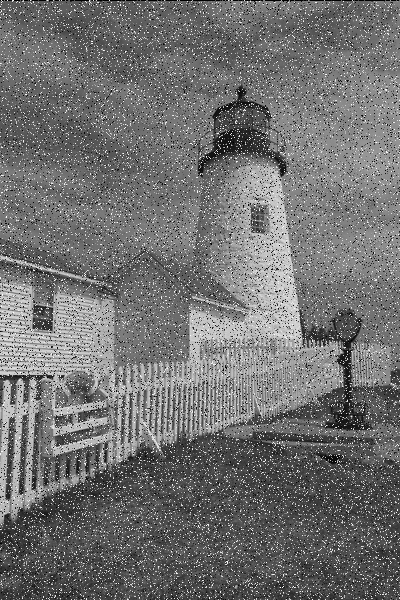
\includegraphics[width=6cm]{ressources/tp4/phare_bruit_ps.png}
      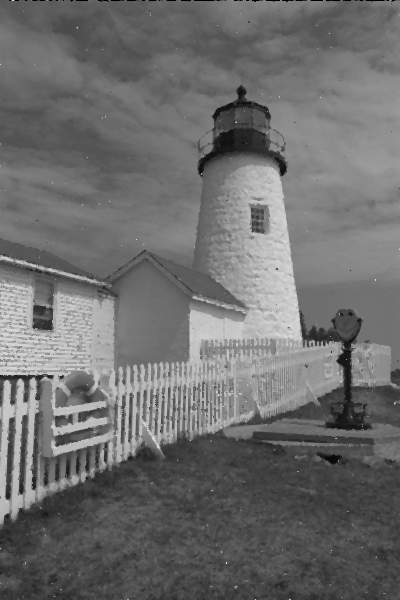
\includegraphics[width=6cm]{ressources/tp4/phare_dest_median.png}
      \caption{Image avant et après l'application du filtre médian}
\end{figure}

Lorsque nous appliquons le filtre moyenneur sur l'image contenant le bruit ``poivre et sel'', nous pouvons constater que l'image
est floutée. Cependant, elle ne contient plus de pixel dont la valeur est très différente de celles des autres pixels qui l'entourent,
contrairement au filtre médian.\\

\subsubsection{Filtre dérivateur}

Nous avons testé ce type de filtre sur une image contrastée sans bruit avec la matrice suivante : 1/2
$\begin{pmatrix}
   0 & 0 & 0\\
   -1 & 0 & 1\\
   0 & 0 & 0
\end{pmatrix}$.
Ce filtre a pour effet de rendre l'image noire avec des traces blanches correspondant aux endroits où il y a une
grosse variation de couleur, soulignant ainsi certains contours.

\begin{figure}[H]
      \center
      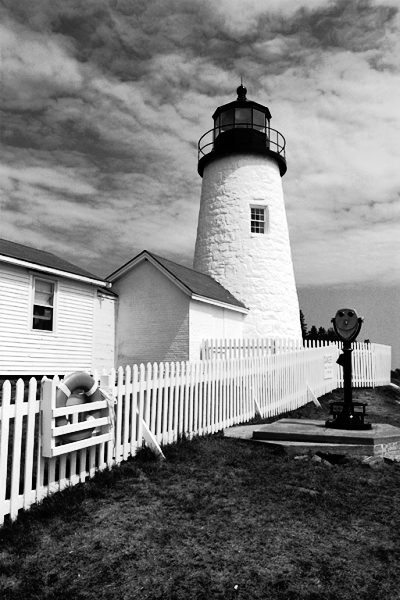
\includegraphics[width=6cm]{ressources/tp4/phare_contraste.png}
      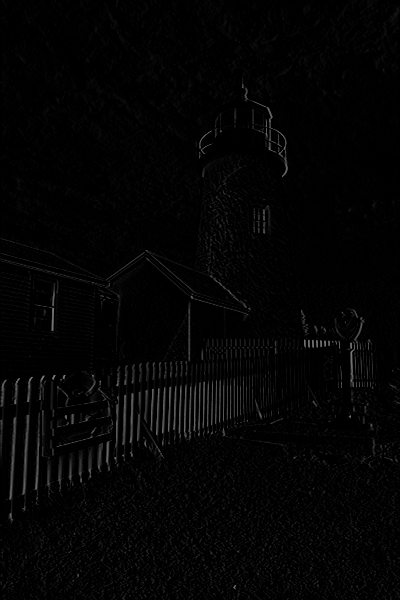
\includegraphics[width=6cm]{ressources/tp4/phare_mat_demi.png}
      \caption{Image avant et après l'application du premier filtre dérivateur}
\end{figure}

Pour obtenir une image qui souligne l'ensemble des contours il nous faut utiliser la matrice suivante : 1/4
$\begin{pmatrix}
   0 & -1 & 0\\
   -1 & 0 & 1\\
   0 & 1 & 0
\end{pmatrix}$.
Cependant, ce filtre va souligner les contours même des plus petits objets comme l'herbe. 

Alors que la matrice 1/8
$\begin{pmatrix}
   0 & 1 & 0\\
   1 & -4 & 1\\
   0 & 1 & 0
\end{pmatrix}$
permet de souligner les contours des objets les plus important.

\begin{figure}[H]
      \center
      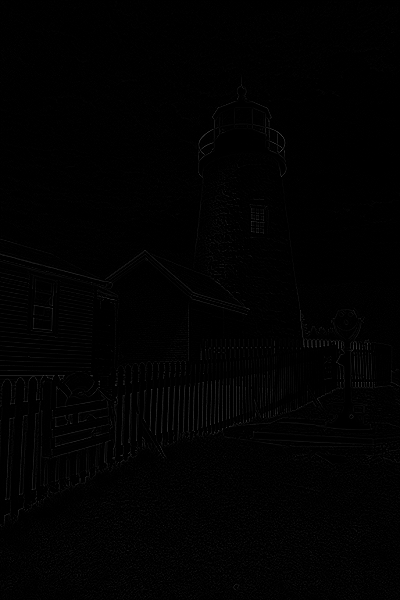
\includegraphics[width=6cm]{ressources/tp4/phare_mat_huit.png}
      \caption{Résultat de la matrice soulignant les contours des objets les plus importants}
\end{figure}

\subsection{Définition et représentation d'histogrammes}

\subsubsection{Exemple d'histogramme 1D avec l'image du phare}
Afin de récupérer davantage d'information sur l'image phare.png, nous avons affiché l'histogramme
de l'image à l'aide d'OpenCV.
\begin{figure}[H]
      \center
      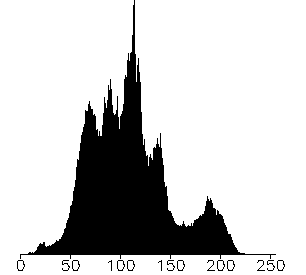
\includegraphics[width=6cm]{ressources/tp4/histo.png}
      \caption{Histogramme de l'image phare.png}
\end{figure}

%On peut voir que les pics les plus sombres correspondent au toit du phare et aux jumelles. 
Les deux premiers pics correspondent au gris présent dans les toits et l'herbe.
Le pic le plus important de l'histogramme représente le ciel qui est en gris et représente une grande partie de l'image. 
Et le dernier pic aux environs de 200 correspond au phare qui est majoritairement blanc.

\subsubsection{Utilisation de l'histogramme sur une image prise par l'interface multitouch}

Nous avons maintenant récupéré l'histogramme d'une image prise avec l'interface multitouch afin 
de déterminer quelle méthode de binarisation est la plus approriée pour notre application.

\begin{figure}[H]
      \center
      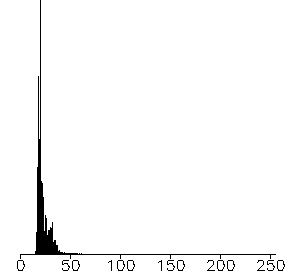
\includegraphics[width=6cm]{ressources/tp4/histoDoigts.png}
      \caption{Histogramme d'une image de la surface multitouch}
\end{figure}

En analysant l'histogramme de cette image on peut voir que l'on ne peut pas déterminer un seuil de 
binarisation car le fond est entièrement noir et il est impossible de distinguer les niveaux de gris des doigts.
Il faudrait donc récupérer l'histogramme d'une ROI\footnote{Region Of Interest} restreinte aux alentours d'un doigt de l'image pour pouvoir déterminer un seuil.

\begin{figure}[H]
      \center
      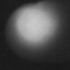
\includegraphics[width=4cm]{ressources/tp4/roi.png}
      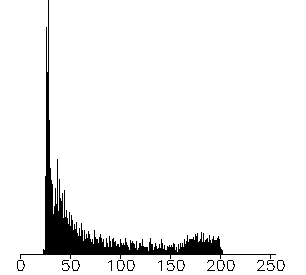
\includegraphics[width=6cm]{ressources/tp4/histoROI.png}
      \caption{Image et histogramme de la ROI d'un doigt}
\end{figure}

On peut voir un pic en debut de l'histogramme qui correspond aux pixels du fond. Mais maintenant 
l'histogramme fait apparaitre les pixels du doigt entre les niveaux de gris 160 et 200 (et du bruit entre les deux zones).
En utilisant 160 en seuil de binarisation avec la méthode \textbf{cvThreshold} nous obtenons une 
image binarisée permettant de bien distinguer les doigts dans l'image.

\begin{figure}[H]
      \center
      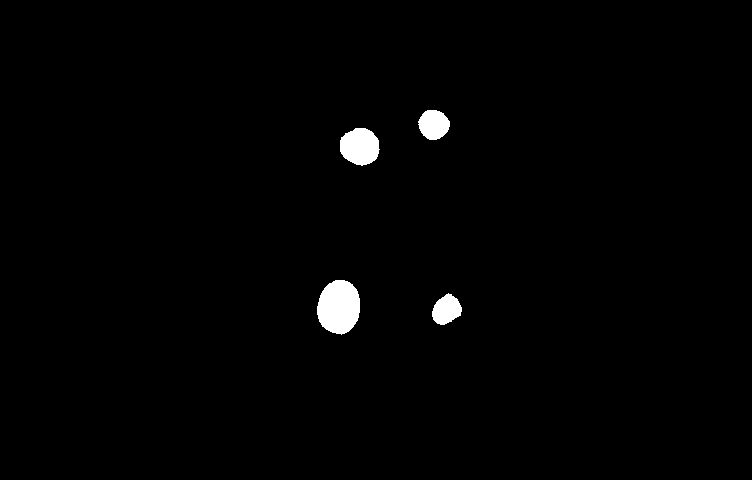
\includegraphics[width=6cm]{ressources/tp4/binarisation.png}
      \caption{Binarisation d'une image provenant de l'interface multitouch}
\end{figure}

En applicant l'option THRESH\_OTSU sur l'image des doigts on obtient une binarisation très satisfesante que l'on 
considère l'image entière ou bien seulement une région restreinte. Les résultats sont très proches. On peut conclure que la méthode d'OTSU est un 
algorithme qui convient à nos besoins et est moins laborieuse qu'une méthode empirique ``à la main''.

\begin{figure}[H]
      \center
      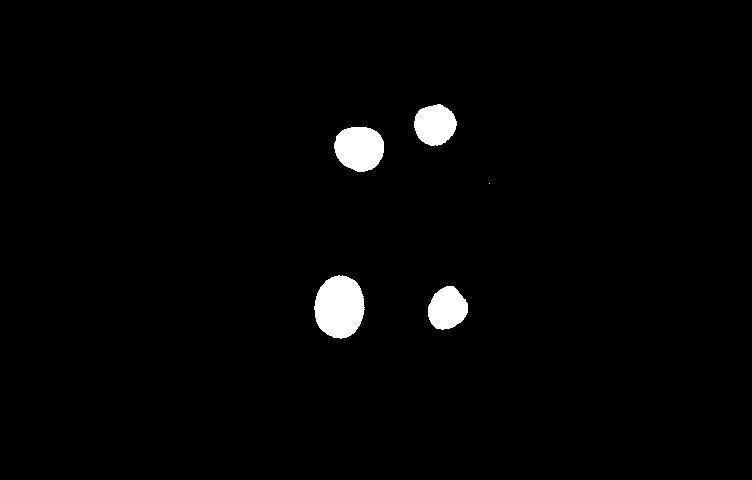
\includegraphics[width=6cm]{ressources/tp4/binarisation_OTSU_ROI.png}
      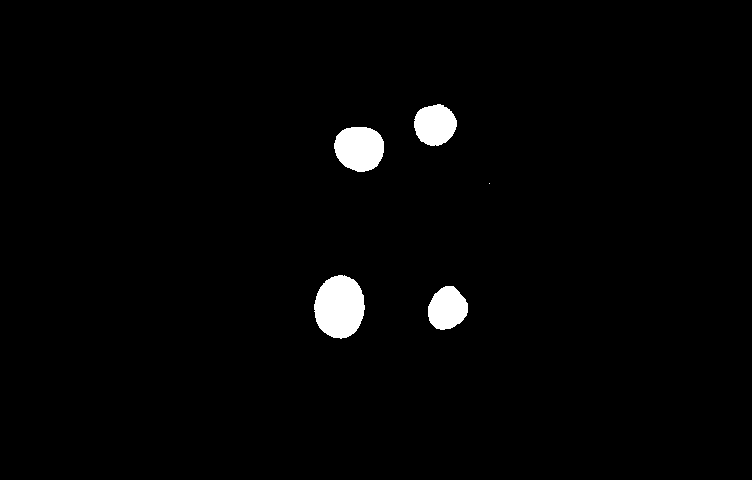
\includegraphics[width=6cm]{ressources/tp4/binarisation_OTSU.png}
      \caption{Comparaison de la binarisation avec la méthode d'OTSU en considérant une ROI restreinte (à gauche) et l'image entière (à droite)}
\end{figure}
